\documentclass[tikz,border=5pt]{standalone}
\usepackage{tikz}
\usepackage{pgfplots}
\usepgfplotslibrary{groupplots}
\pgfplotsset{compat=1.18}
% sha256: 908b490fa62a6a14ea628a5bd963bb8d77f3673efc8c014d964d06120217f0be
\definecolor{p06color0}{HTML}{0072B2}
\definecolor{p06color1}{HTML}{E69F00}
\definecolor{p06color2}{HTML}{000000}
\begin{document}
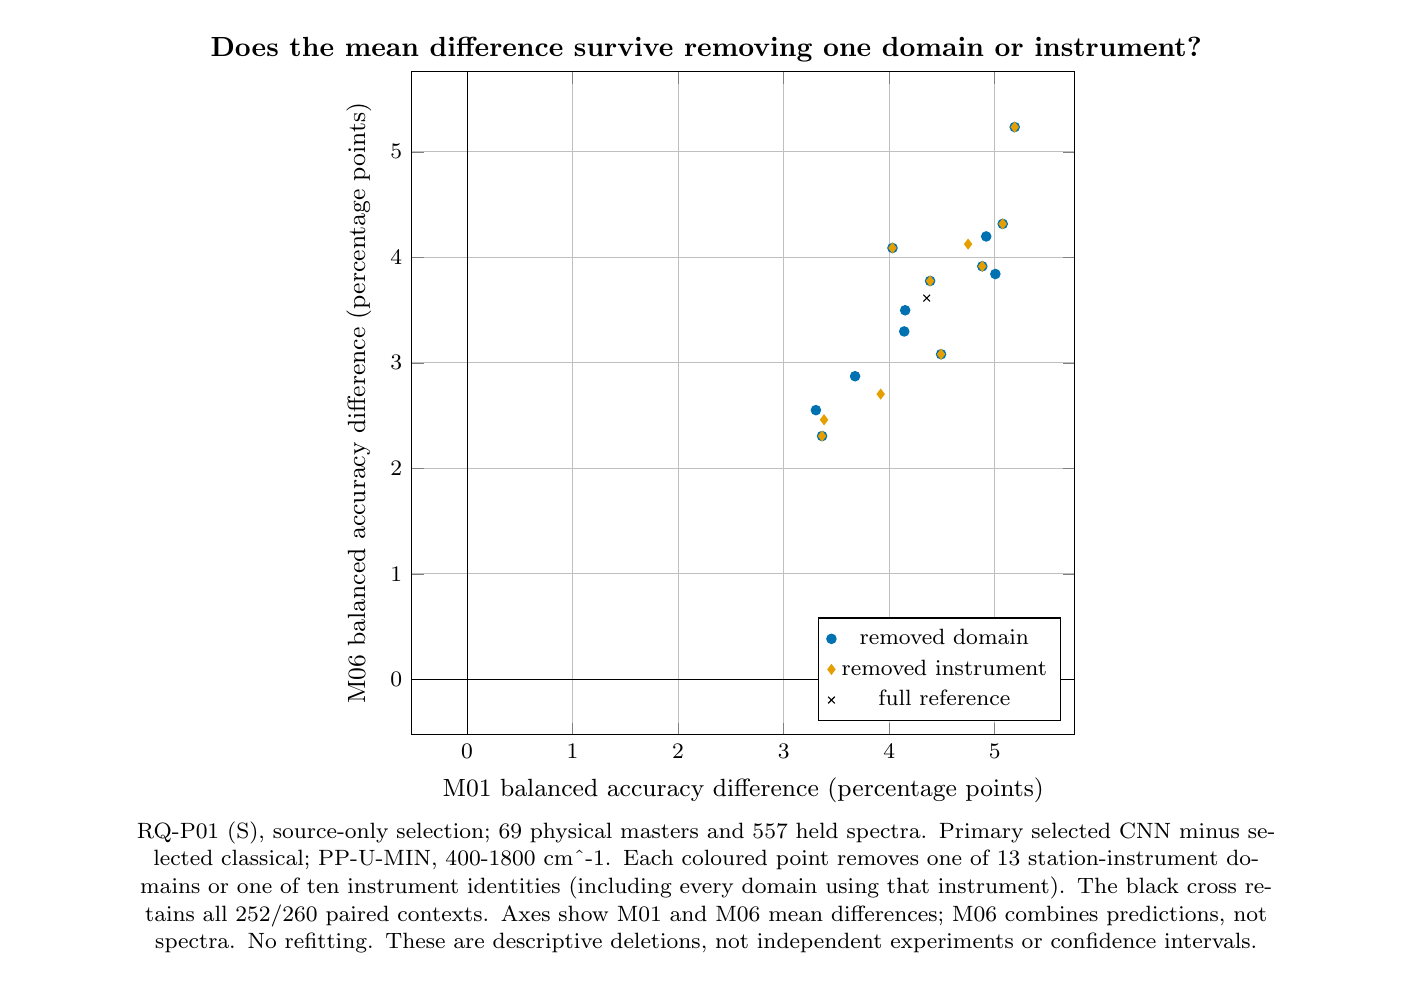
\begin{tikzpicture}
\begin{groupplot}[group style={group size=1 by 1, horizontal sep=1.8cm},
width=10cm,
height=10cm,
xmin=-0.523432423651722, xmax=5.75775666016894, ymin=-0.523432423651722, ymax=5.75775666016894,
xlabel={M01 balanced accuracy difference (percentage points)},
xlabel style={font=\fontsize{9}{11}\selectfont, color=black},
ylabel={M06 balanced accuracy difference (percentage points)},
ylabel style={font=\fontsize{9}{11}\selectfont, color=black},
tick label style={font=\fontsize{8}{10}\selectfont, color=black},
title style={font=\bfseries\fontsize{10}{12}\selectfont, color=black},
grid=both,
axis equal]
\nextgroupplot[title={}, legend style={at={(0.98,0.02)},anchor=south east,draw=black,fill=white,font=\fontsize{8}{10}\selectfont}]
\addplot[forget plot, black, thin] coordinates {(0,-0.523432423651722) (0,5.75775666016894)};
\addplot[forget plot, black, thin] coordinates {(-0.523432423651722,0) (5.75775666016894,0)};
\addplot[only marks, mark=*, mark size=1.7pt, color=p06color0] coordinates {(5.18929733494793,5.23432423651722) (5.0060008150286,3.8417803768681) (5.07585136733529,4.3169265756985) (4.03120851019243,4.08849090318389) (4.1515788805628,3.49821312540611) (4.38785533558926,3.77599090318389) (4.49185665834058,3.08154645873944) (3.67704184352577,2.87321312540611) (4.91932579414305,4.19780160277236) (3.36404581177973,2.30608349577648) (3.30556918038644,2.55171106779294) (4.14257682294964,3.29759584145549) (4.88229376752769,3.91487979207277)};
\addlegendentry{removed domain}
\addplot[only marks, mark=diamond*, mark size=1.7pt, color=p06color1] coordinates {(4.03120851019243,4.08849090318389) (4.74785036128737,4.12487447575167) (3.36404581177973,2.30608349577648) (5.18929733494793,5.23432423651722) (4.38785533558926,3.77599090318389) (4.49185665834058,3.08154645873944) (3.91948525660647,2.70393998464174) (3.38281107958142,2.46101364522417) (5.07585136733529,4.3169265756985) (4.88229376752769,3.91487979207277)};
\addlegendentry{removed instrument}
\addplot[only marks, mark=x, mark size=1.7pt, color=p06color2] coordinates {(4.35573093248532,3.61373519268256)};
\addlegendentry{full reference}
\end{groupplot}
\node[anchor=south, font=\bfseries\fontsize{10}{12}\selectfont] at (current bounding box.north) {Does the mean difference survive removing one domain or instrument?};
\node[anchor=north, text width=17cm, align=center, font=\fontsize{8}{10}\selectfont] at (current bounding box.south) {RQ-P01 (S), source-only selection; 69 physical masters and 557 held spectra. Primary selected CNN minus selected classical; PP-U-MIN, 400-1800 cm\textasciicircum{}-1. Each coloured point removes one of 13 station-instrument domains or one of ten instrument identities (including every domain using that instrument). The black cross retains all 252/260 paired contexts. Axes show M01 and M06 mean differences; M06 combines predictions, not spectra. No refitting. These are descriptive deletions, not independent experiments or confidence intervals.};
\end{tikzpicture}
\end{document}
